\chapter{Supporting Information: Chaotic but regular recurrent
  influenza epidemics: from theory to observation}

%other title proposals
%\title{Chaotic dynamics with uniform phase in influenza
%  epidemics: from theory to observation}


Sébastien Ballesteros$^{1,*}$, 
Lewi Stone$^{2}$,
Anton Camacho$^{1}$,
Elisabeta Vergu$^{3}$,
Bernard Cazelles$^{1,4}$

\vspace{2cm}

$^1$UMR 7625  (UPMC, ENS, AgroParisTech, CNRS), Ecole Normale
Supérieure, Unit of Eco-Evolutionary Mathematics,  46 rue d'Ulm,
F-75230 Paris Cedex 05, France. \\
$^2$Biomathematics Unit, Faculty of Life Sciences, Tel Aviv
University, Ramat Aviv 69978, Israel \\
$^3$~INRA, UR341 Mathématiques et Informatique Appliquées, F-78352 Jouy en Josas, France \\
$^4$~UMMISCO UMI 209 IRD-UPMC, F-93142 Bondy, France.

~\\
$^*$\textit{Corresponding author}:  \\
E-mail: sebastien.ballesteros@biologie.ens.fr

%\tableofcontents

\section{Models}

\subsection{A minimal model for two subtypes of influenza A interacting
    via a short period of full cross-immunity}

  Fig.~\ref{fig:2subtypes} presents a schematic representation of
  the model described by eq. 2 in the main manuscript, for the two-subtype case.
 
\begin{figure}[htbp]
  \center
  \begin{tikzpicture}[node distance=2cm, inner sep=0pt, minimum size=10mm]
    
    \tikzstyle{seb}=[rectangle, fill=red, draw=gray, text=black] \tikzstyle{I1}=[->,   draw=red, shorten >=1pt, >=stealth',semithick]                     \tikzstyle{I2}=[->,draw=blue, shorten >=1pt, >=stealth',semithick] \tikzstyle{g1}=[->,shorten >=1pt, >=stealth',semithick]                     \tikzstyle{g2}=[->,shorten >=1pt, >=stealth',semithick]
    
    \node[seb] (R0) {$R_\varnothing$}; \node[seb] (R1) [above of=R0] {$R_1$}; \node[seb] (R2) [below of=R0] {$R_2$}; \node[seb] (R12) [right                    of=R0] {$R_{12}$};
    
    \draw[I1] (R0) to node[auto] {\begin{tiny}$\beta(t) R_\varnothing
        (I^1 +\eta_1)$, $\nu     I_\varnothing^1$, $qQ_1$\end{tiny}} (R1) ;
    \draw[I2] (R0) to node[auto,swap] {\begin{tiny}$\beta(t)
        R_\varnothing  (I^2 +\eta_2)$, $\nu     I_\varnothing^2$, $qQ_2$\end{tiny}} (R2);
    \draw[I2] ([yshift=+4mm] R1.east) to node[auto]
    {\begin{tiny}$\beta(t) R_1 (I^2 +\eta_2)$, $\nu     I_1^2$, $qQ_{12}$\end{tiny}} ([yshift=+4mm] R12.west) ;
    \draw[I1] ([yshift=-4mm] R2.east) to node[auto,swap]
    {\begin{tiny}$\beta(t) R_2 (I^1 +\eta_1)$,     $\nu I_2^1$, $qQ_{12}$\end{tiny}} ([yshift=-4mm] R12.west) ;
    \draw[g1] ([xshift=+2mm] R1.south) to node[auto] {\begin{tiny}$g$ $g$\end{tiny}} ([xshift=+2mm] R0.north) ;
    \draw[g2] ([xshift=+2mm] R2.north) to node[auto,swap] {\begin{tiny}$g$ $g$\end{tiny}} ([xshift=+2mm] R0.south) ;
    \draw[g1] (R12.west) to (R2.east) ;
    \draw[g2] (R12.west) to (R1.east) ;
  \end{tikzpicture}
  \caption{A minimal model for two subtypes of influenza A interacting
    via a short period of full cross-immunity ($Q$) of average
    duration $1/q$. With the notation of eq. 2 of the main manuscript, $J=\{\{\varnothing\},
    \{1\}, \{2\}, \{1,2\}\}$ and indicates the current level of immunity;
    $k$ indexes the co-circulating subtypes ($k=1, 2$).  Infection
    (transition from states $R_{J\setminus k}$ to $R_J$) are
    represented by red and blue arrows for subtypes 1 and 2. During
    the transition, hosts pass through states $I^k_{J\setminus k}$ and
    $Q_J$ as indicated on the arrows.  As the viral population evolves,
    hosts can loose immunity (black arrows).}
  \label{fig:2subtypes}
\end{figure}

\clearpage

\subsection{Stochastic metapopulation model with age structure}

Eq. 2 (main manuscript) was extended to a stochastic metapopulation model of 52 cities
depicted in Fig.~\ref{fig:iata} and indexed by $c_l$ in the equations
below.

\begin{figure}[htb]
  \center
  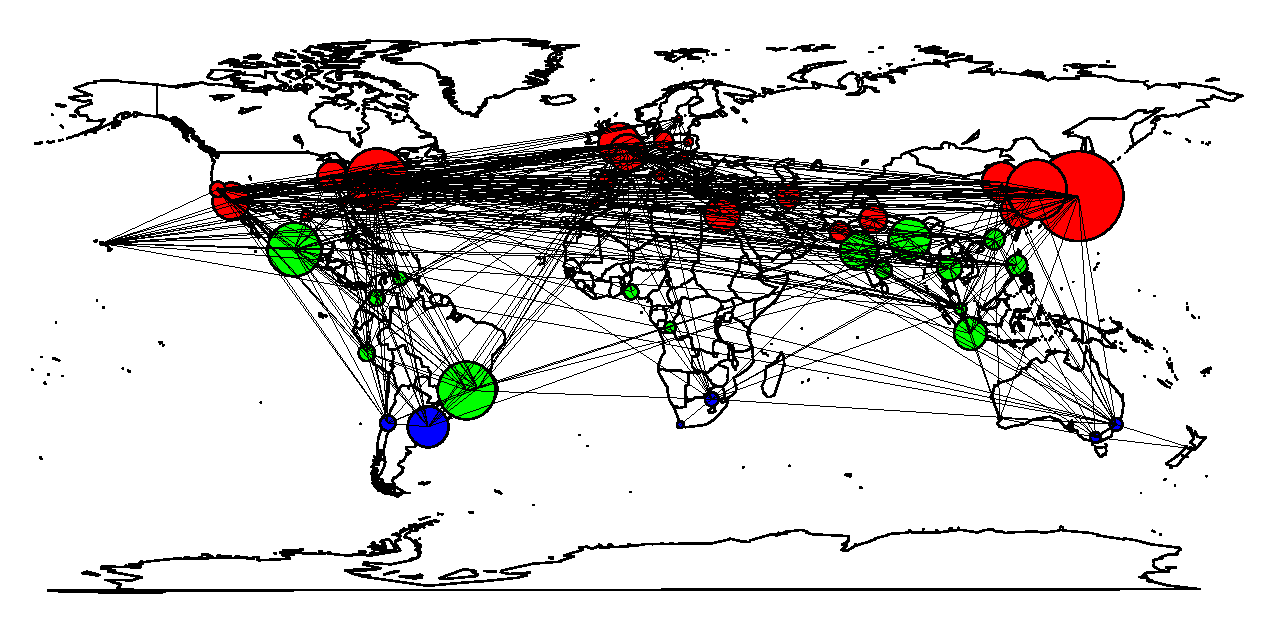
\includegraphics[width= 0.8 \linewidth]{texte/article2/graph_annexe/iata.eps}
  \caption{Overview of the network of 52 major cities used in the
    stochastic metapopulation model. Circle areas and connection lines width are
    proportional to city sizes and air transportation flows respectively. Red,
    green and blue indicate the three geographic area used (North,
    Tropics, South respectively).}
  \label{fig:iata}
\end{figure}


\begin{footnotesize}
\begin{align}
%  \label{eq:app2:full}
%%R
\dot{R}_{\begin{subarray}{l}J\\ a_i, c_l \end{subarray}} &=  q Q_{\begin{subarray}{l}J  \\ a_i,
    c_l \end{subarray}} - \sum_{k \notin J} \sigma_{a_i}^k \beta_k(t)
\frac{R_{\begin{subarray}{l}J\\ a_i, c_l \end{subarray}}}{p_{a_i} N_{c_l}} \sum_j M_{ij}
I^k_{a_j,c_l} -\sum_{k
  \in J} g_k R_{\begin{subarray}{l}J\\ a_i, c_l \end{subarray}} + \sum_{k
  \notin J} g_k R_{\begin{subarray}{l}J \cup k \\ a_i, c_l \end{subarray}} \notag \\
%%
%%E
\dot{E_1}^k_{\begin{subarray}{l}J \setminus k\\ a_i,
    c_l \end{subarray}} &=\sigma_{a_i}^k \beta_k(t)
\frac{R_{\begin{subarray}{l}J \setminus k\\ a_i, c_l \end{subarray}}}{p_{a_i} N_{c_l}} \sum_j M_{ij}
I^k_{a_j,c_l} -2 \gamma {E_1}^k_{\begin{subarray}{l}J
    \setminus k\\ a_i, c_l \end{subarray}} -\sum_{m\neq l}
\frac{p_{a_i} \tau_{c_lc_m}}{N_{c_l}} {E_1}^k_{\begin{subarray}{l}J \setminus k\\ a_i,
    c_l \end{subarray}} -\sum_{m
  \in J \setminus k} g_m {E_1}^k_{\begin{subarray}{l}J \setminus k\\ a_i, c_l \end{subarray}} + \sum_{m
  \notin J \setminus k} g_m {E_1}^k_{\begin{subarray}{l} (J \setminus k) \cup m \\ a_i, c_l \end{subarray}} 
\notag \\
%%
%%E'
\dot{E_2}^k_{\begin{subarray}{l}J \setminus k\\ a_i, c_l \end{subarray}}
&=2 \gamma {E_1}^k_{\begin{subarray}{l}J \setminus k\\ a_i,
    c_l \end{subarray}} -2 \gamma {E_2}^k_{\begin{subarray}{l}J \setminus k\\ a_i, c_l \end{subarray}}
+\sum_{m\neq l} \frac{p_{a_i} \tau_{c_mc_l}}{N_{c_l}} {E_1}^k_{\begin{subarray}{l}J \setminus k\\ a_i,
    c_m \end{subarray}} -\sum_{m\neq l} \frac{p_{a_i}  \tau_{c_lc_m}}{N_{c_l}} {E_2}^k_{\begin{subarray}{l}J \setminus k\\ a_i,
    c_l \end{subarray}} -\sum_{m
  \in J \setminus k} g_m {E_2}^k_{\begin{subarray}{l}J \setminus k\\ a_i, c_l \end{subarray}} + \sum_{m
  \notin J \setminus k} g_m {E_2}^k_{\begin{subarray}{l} (J \setminus k) \cup m \\ a_i, c_l \end{subarray}}  \notag \\
%%
%%I
\dot{I_1}^k_{\begin{subarray}{l}J \setminus k\\ a_i, c_l \end{subarray}} &=2 \gamma {E_2}^k_{\begin{subarray}{l}J \setminus k\\ a_i, c_l \end{subarray}}
-2 \nu {I_1}^k_{\begin{subarray}{l}J \setminus k\\ a_i,
    c_l \end{subarray}} + \sum_{m\neq l} \frac{p_{a_i} \tau_{c_mc_l}}{N_{c_l}} {E_2}^k_{\begin{subarray}{l}J \setminus k\\ a_i,
    c_m \end{subarray}}  -\sum_{m
  \in J \setminus k} g_m {I_1}^k_{\begin{subarray}{l}J \setminus k\\ a_i, c_l \end{subarray}} + \sum_{m
  \notin J \setminus k} g_m {I_1}^k_{\begin{subarray}{l} (J \setminus k) \cup m \\ a_i, c_l \end{subarray}}  \notag \\
%%
%%I'
\dot{I_2}^k_{\begin{subarray}{l}J \setminus k\\ a_i,
    c_l \end{subarray}} &=2 \nu {I_1}^k_{\begin{subarray}{l}J:k
    \notin J\\ a_i, c_l \end{subarray}} -2 \nu {I_2}^k_{\begin{subarray}{l}J \setminus k\\ a_i, c_l \end{subarray}} -\sum_{m
  \in J \setminus k} g_m {I_2}^k_{\begin{subarray}{l}J \setminus k\\ a_i, c_l \end{subarray}} + \sum_{m
  \notin J \setminus k} g_m {I_2}^k_{\begin{subarray}{l} (J \setminus k) \cup m \\ a_i, c_l \end{subarray}} 
\notag \\
%%
%%Q
\dot{Q}^k_{\begin{subarray}{l}J \\ a_i, c_l \end{subarray}}
&= \sum_{k \in J} 2 \nu {I_2}^k_{\begin{subarray}{l}J \setminus k\\
    a_i,
    c_l \end{subarray}} - q Q_{\begin{subarray}{l}J \\
    a_i, c_l \end{subarray}} -\sum_{k \in J} g_k
Q_{\begin{subarray}{l}J\\ a_i, c_l \end{subarray}} + \sum_{k \notin J}
g_k Q_{\begin{subarray}{l}J \cup k \\ a_i, c_l \end{subarray}} \notag
\end{align}
\end{footnotesize}

where $\frac{p_{a_i} \tau_{c_mc_l}}{N_{c_l}}$ are probabilities that a
host of age class $a_i$ situated in city $c_l$ of size $N_{c_l}$
travels from city $c_l$ to city $c_m$ (value given in
\citep{Grais2003}).  Three age classes ($a_i$) were considered, with $a_1 =$
0-19 years old, $a_2 =$ 20-59 years old and $a_3 \geq$ 60 years
old. City specific population sizes ($N_{c_l}$) and age distributions $p_{a_i}$ were
taken from
https://www.cia.gov/library/publications/the-world-factbook/ and
http://unstats.un.org/unsd/demographic/. To increase realism, exposed
period was added ($E$) and exposed and infectious classes were doubled
($E_1$, $E_2$ and $I_1$, $I_2$) to ensure that the exposed and
infectious period followed Erlang distributions (which are more realistic than memoryless exponential distributions usually employed for sojourn times).  Following
\citet{Cooper2006a} it was assumed that only exposed individuals
traveled.

\subsection{Numerical Methods}

Eq.~1 and 2 (of the main manuscript) were integrated by a Runge Kutta method of order 4-5 with adaptive
time step algorithm provided by the C library GSL \citep{Galassi2003}.

The stochastic metapopulation model was integrated using an
Euler-multinomial approximation of the continuous-time Markov process
\citep{Breto2009} written in C and using library GSL
\citep{Galassi2003} for random number generation and distribution.

\clearpage

\section{Parameter inference}

\subsection{Methods}

To compare the UPCA model to real data, we have implemented a
stochastic version of eq.~1 model described in the main manuscript using an Euler-multinomial approximation to the
continuous-time Markov process. A dephasing term $d$ was added to the
seasonal forcing function: $\beta(t)=\beta_0(1+e \cos(2 \pi t +d
2\pi)$. 

We have contrasted the realisation of the process model ($x_t$) with
weekly incidence data ($y_t$).

Two data sets were used: weekly incidence rates for Influenza Like
Illness (ILI) of region Ile de France (Paris and its surrounding area) from
the French Sentinelles network and daily ILI data for Israel (LEWI, source). The French
Sentinelles data (http://websenti.b3e.jussieu.fr/sentiweb/) correspond to consultations for ILI declared by a network of volunteer general practitioners.  As the
data come normalised per 100 000 hosts, we have followed
\citep{Finkenstaedt2005} and kept the population size fixed to 100 000
hosts.
For Israel, the population size was taken equal to 1822438 LEWI,source 

Simulated weekly incidence rates were computed as
$x_t=\int_{t-1}^t \nu I(t) dt$ and contrasted to the real weekly
reported incidence, $y_t$, with an observation process characterized by a
reporting rate ($\rho$). We set $Y_t | \rho_t,x_t \sim P(\rho_t,x_t)$
(where $P$ stands for the Poisson distribution) and, to account for
Overdispersion, we allow variability in the reporting rate by assuming
that $\rho_t \sim \Gamma(\frac{1}{\phi}, \rho \phi)$ (where $\Gamma$
is the gamma distribution).  The observation process is then fully
described by a negative binomial distribution ($NB$): $Y_t | x_t \sim
NB(\mathrm{mean}=\rho x_t, \mathrm{size}=\frac{1}{\phi})$.

Parameter inference was achieved through an implementation of a maximum
likelihood approach via iterated filtering (MIF) \citep{Ionides2006, Breto2009}
written in C, using the standalone math library from R \citep{R2008}
for random number generation and distribution.

%We used a log transform for positive parameters and a logit transform
%for parameters lying in the interval $[0, 1]$.


\subsection{Results for Ile de France data}

The results of the inference procedure are presented in
Fig.~\ref{fig:profile}.

\begin{figure}[htb]
  \center
    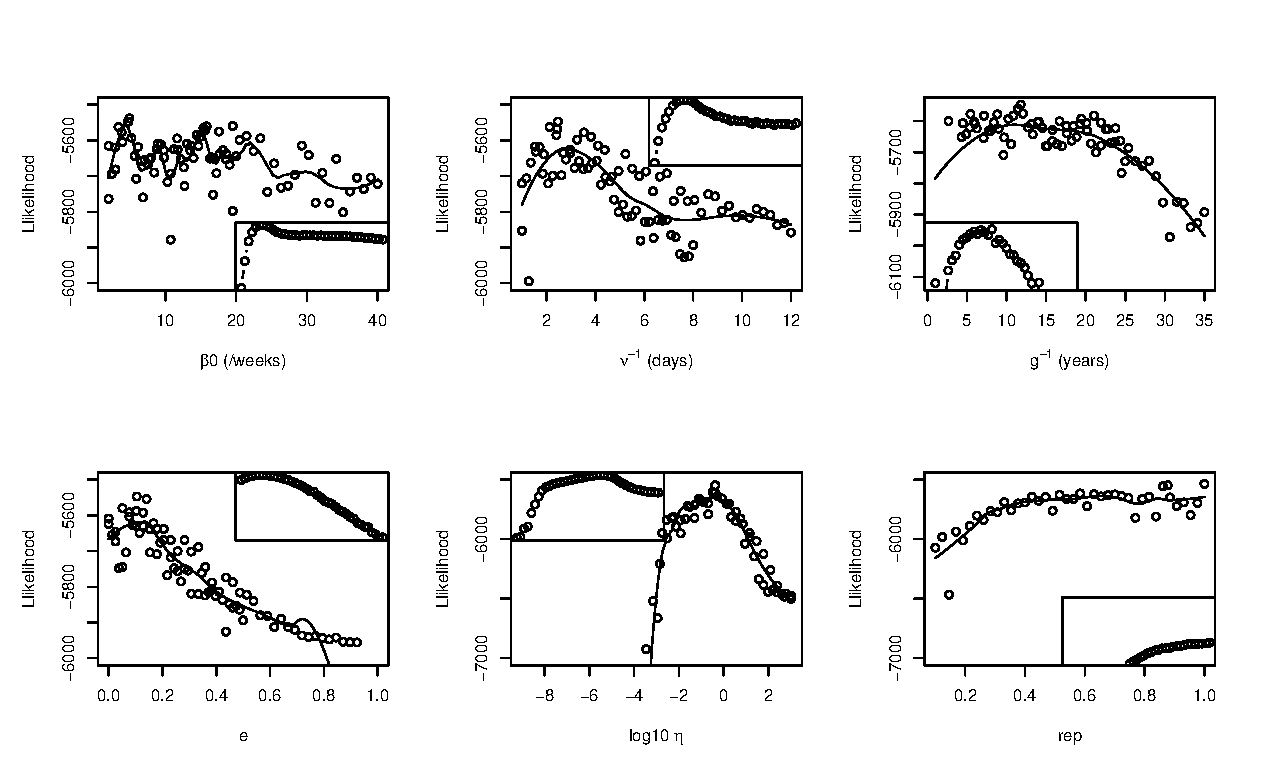
\includegraphics[width= 0.9 \linewidth]{texte/article2/graph_annexe/profile.eps}
    \caption{Likelihood profiles (likelihood value following the
      evolution of a focal parameter, the others parameters being
      re-estimated by MIF) and likelihood slices (likelihood value
      fixing the value of all but the focal parameter at their maximum
      likelihood estimate) (inset). A stochastic version of the single
      subtype model with an observation process following a negative
      binomial distribution is fitted to the ILI French Sentinelles
      network data for Ile de France region. Two replications with
      different initial condition and algorithm parameters are plotted
      and local quadratic regression is used to estimate the profile
      likelihood.}
  \label{fig:profile}
\end{figure}

A strong correlation between $\beta_0$ and $g$ was found as reported in Fig.
\ref{fig:cor}.

% As most of the estimate for $R_0$ are between 1.5 and 2
% \citep{Lessler2007} we fixed $R_0$ to its best estimates of 1.65.

\begin{figure}[htb]
  \center
    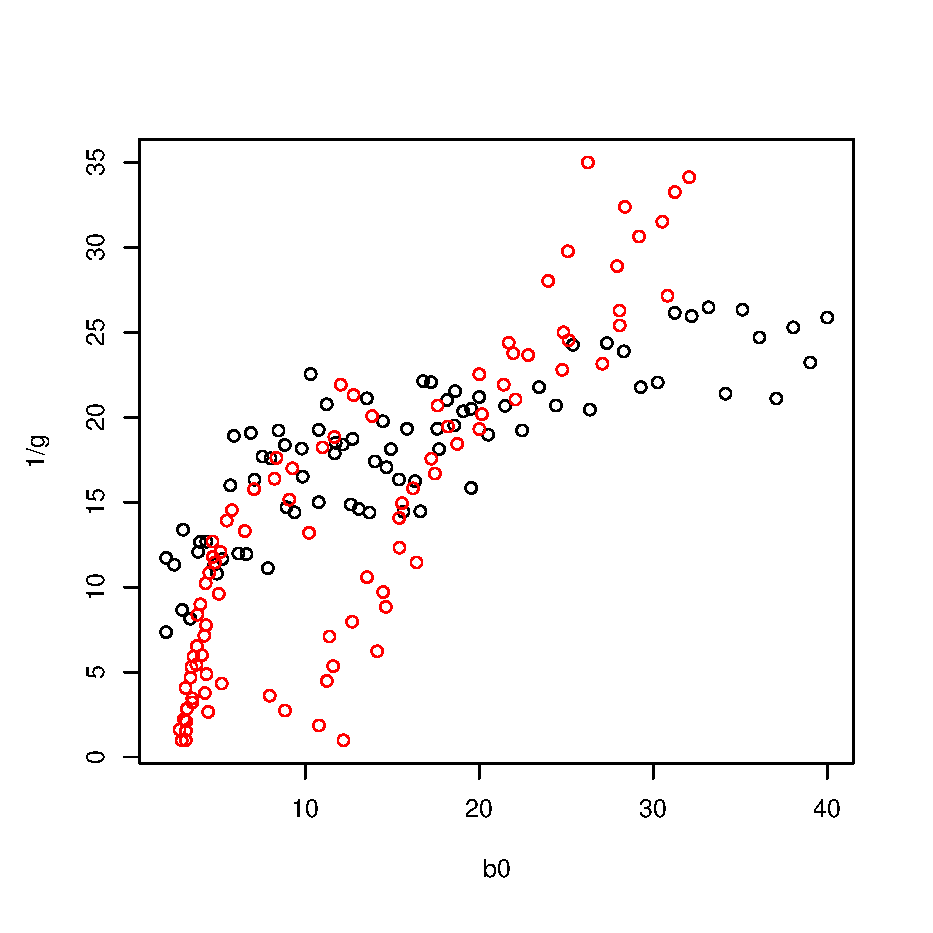
\includegraphics[width= 0.5 \linewidth]{texte/article2/graph_annexe/corr_g_b0.eps}
    \caption{Correlation between $\beta_0$ and $g$ calculated for two
      replications with different initial condition and 
      parameters. Black: $\beta_0$ is fixed and the inferred value of
      $g$ is plotted. Red: $g$ is fixed and the inferred value of
      $\beta_0$ is plotted. For each case, the other parameters are
      re-estimated to their maximum likelihood value. }
  \label{fig:cor}
\end{figure}

\clearpage

\subsection{Results for Israel data}


\begin{figure}[htb]
  \center
    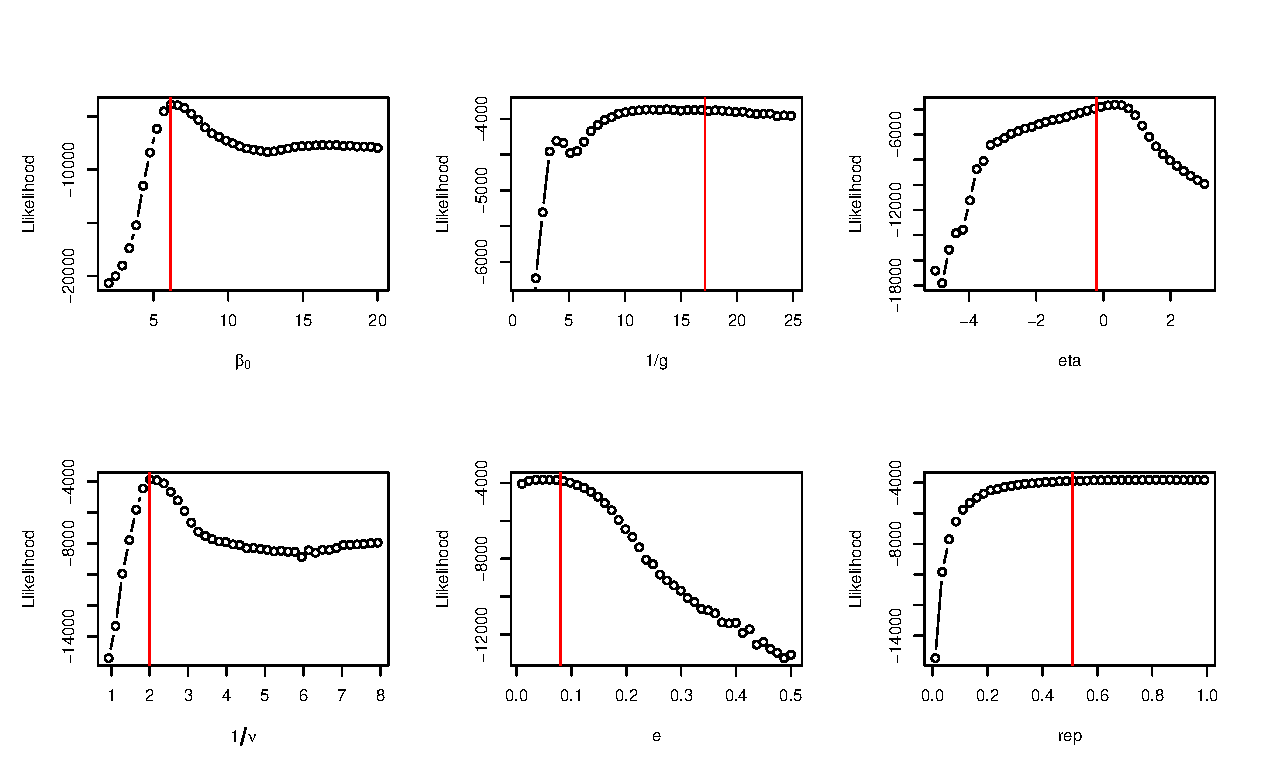
\includegraphics[width= 0.9 \linewidth]{texte/article2/graph_annexe/slice_israel.eps}
    \caption{Likelihood slice}
  \label{fig:israel}
\end{figure}




%\clearpage

\section{Additional figures}

%\subsection{Single subtype model}

\begin{figure}[htbp]
  \center
  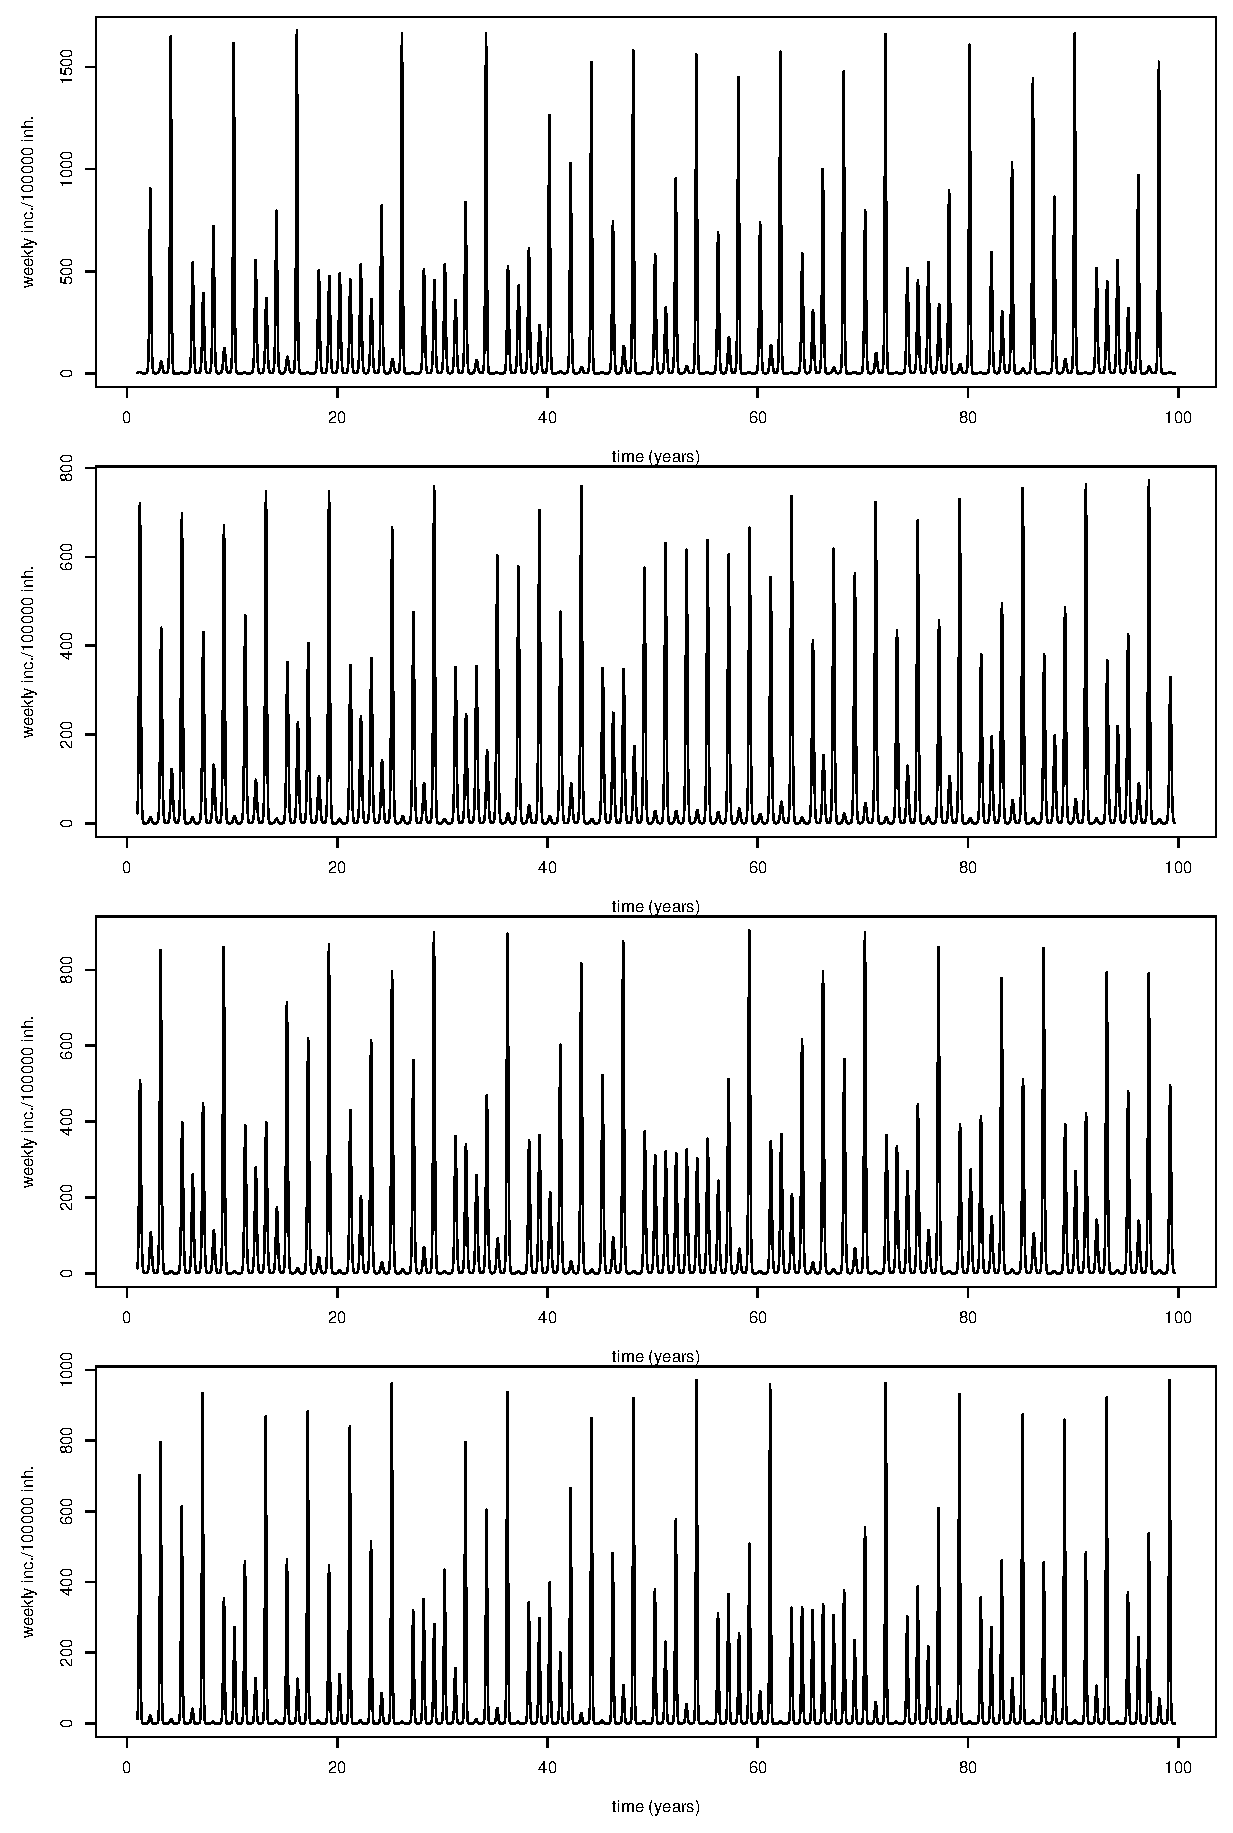
\includegraphics[width= 0.8 \linewidth]{texte/article2/graph_annexe/1strain_traj100.eps}
  \caption{Additional trajectories for the single subtype deterministic UPCA model. Weekly
    incidences per 100 000 inhabitants are plotted.
    First line: $R_0=1.65$, $1/v=2.47$ days$^{-1}$, $1/g=7$
    years$^{-1}$, $e=0.104$, $\eta=10^{-6.7}$ ;
    Second line: $R_0=1.65$, $1/v=2.47$ days$^{-1}$, $1/g=11$
    years$^{-1}$, $e=0.104$, $\eta=10^{-7}$ ;
    Third line: $R_0=5$, $1/v=8$ days$^{-1}$, $1/g=20$ years$^{-1}$,
    $e=0.35$, $\eta=10^{-6}$ ;
    Fourth line: $R_0=2.66$, $1/v=2.77$ days$^{-1}$, $1/g=20$ years$^{-1}$, $e=0.2$, $\eta=10^{-7}$
  }
\label{fig:1strain_traj100}
\end{figure}

%\clearpage

%\subsection{Two-subtype models}

\begin{figure}[htb]
  \center
  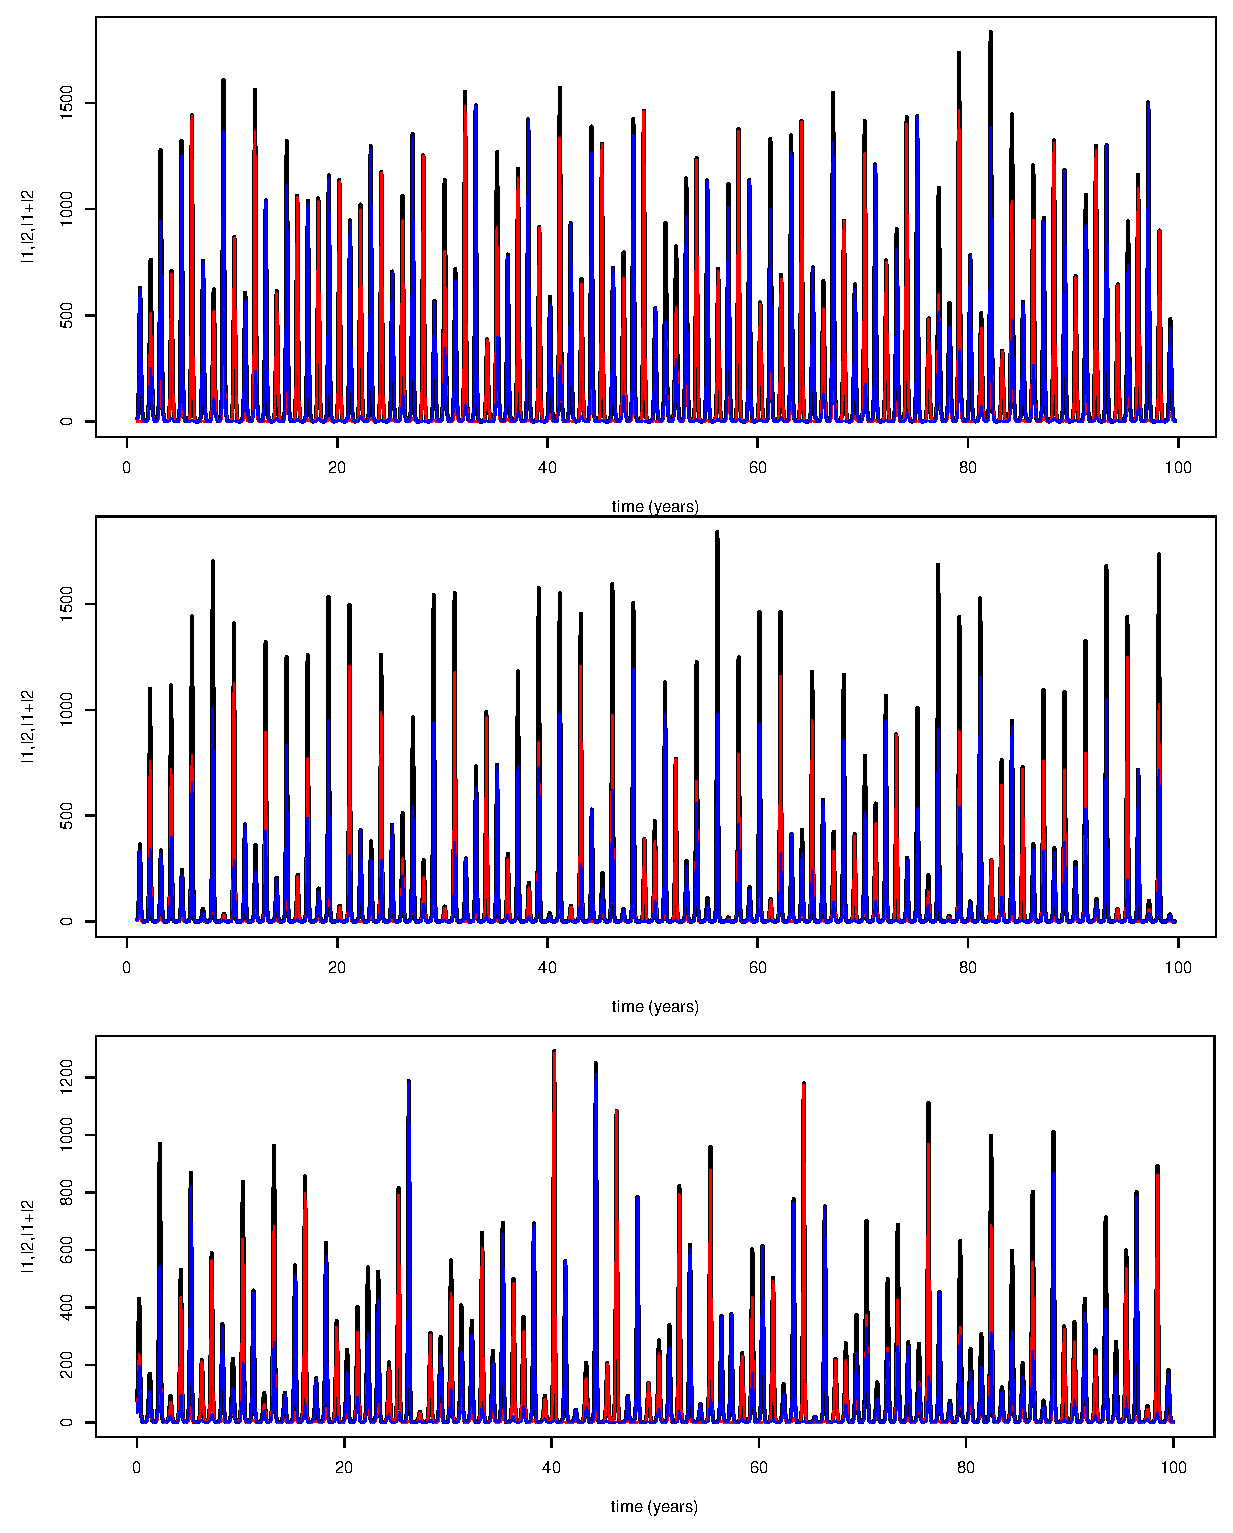
\includegraphics[width= 0.8 \linewidth]{texte/article2/graph_annexe/2strain_traj100.eps}
  \caption{Additional trajectories for two-subtype deterministic
    (first and second line) and stochastic metapopulation UPCA model (third line). Blue and red lines
    are weekly incidence per 100 000 inhabitants for subtypes 1 and 2
    and black lines correspond to the sum of both.
    First line: $R_0=5$, $1/v=8$ days$^{-1}$, $1/g=15$ years$^{-1}$,
    $1/q=6$ months$^{-1}$, $e=0.35$, $\eta=10^{-6}$ ;
    Second line: $R_0=2.66$, $1/v=2.77$ days$^{-1}$, $1/g=20$
    years$^{-1}$, $1/q=6$ months$^{-1}$, $e=0.2$, $\eta=10^{-7}$ ;
    Third line: Typical realisation for the city of Paris $R_0=2.66$, $1/v=2.77$ days$^{-1}$, $1/ \gamma=1.5$
    days$^{-1}$),  $1/g=25$ years$^{-1}$, $1/q=6$ months$^{-1}$, $e=0.2$
  }
  \label{fig:2strain_traj100}
\end{figure}

%\clearpage

%\subsection{Metapopulation model}

\begin{figure}[htb]
  \center
  \includegraphics[width= 0.8 \linewidth]{texte/article2/graph_annexe/world_upca_aggreg.eps}
  \caption{Twenty realisations of the stochastic metapopulation model
    aggregated by geographic areas. Blue and red lines are weekly
    incidence per 100 000 inhabitants for subtypes 1 and 2 and black
    lines correspond to the sum of both. Parameters are those of the empirical
    parameter set (Table 1 in the main manuscript). The remaining parameters are set equal to $1/g=25$ years$^{-1}$, $1/q=6$ months$^{-1}$,
    $1/ \gamma=1.5$ days$^{-1}$. Seasonal forcing ($e=0.2$) for
    Northern and Southern hemisphere are in phase opposition
    and Tropics do not present seasonality. }
  \label{fig:world_aggreg}
\end{figure}

\begin{figure}[htb]
  \center
  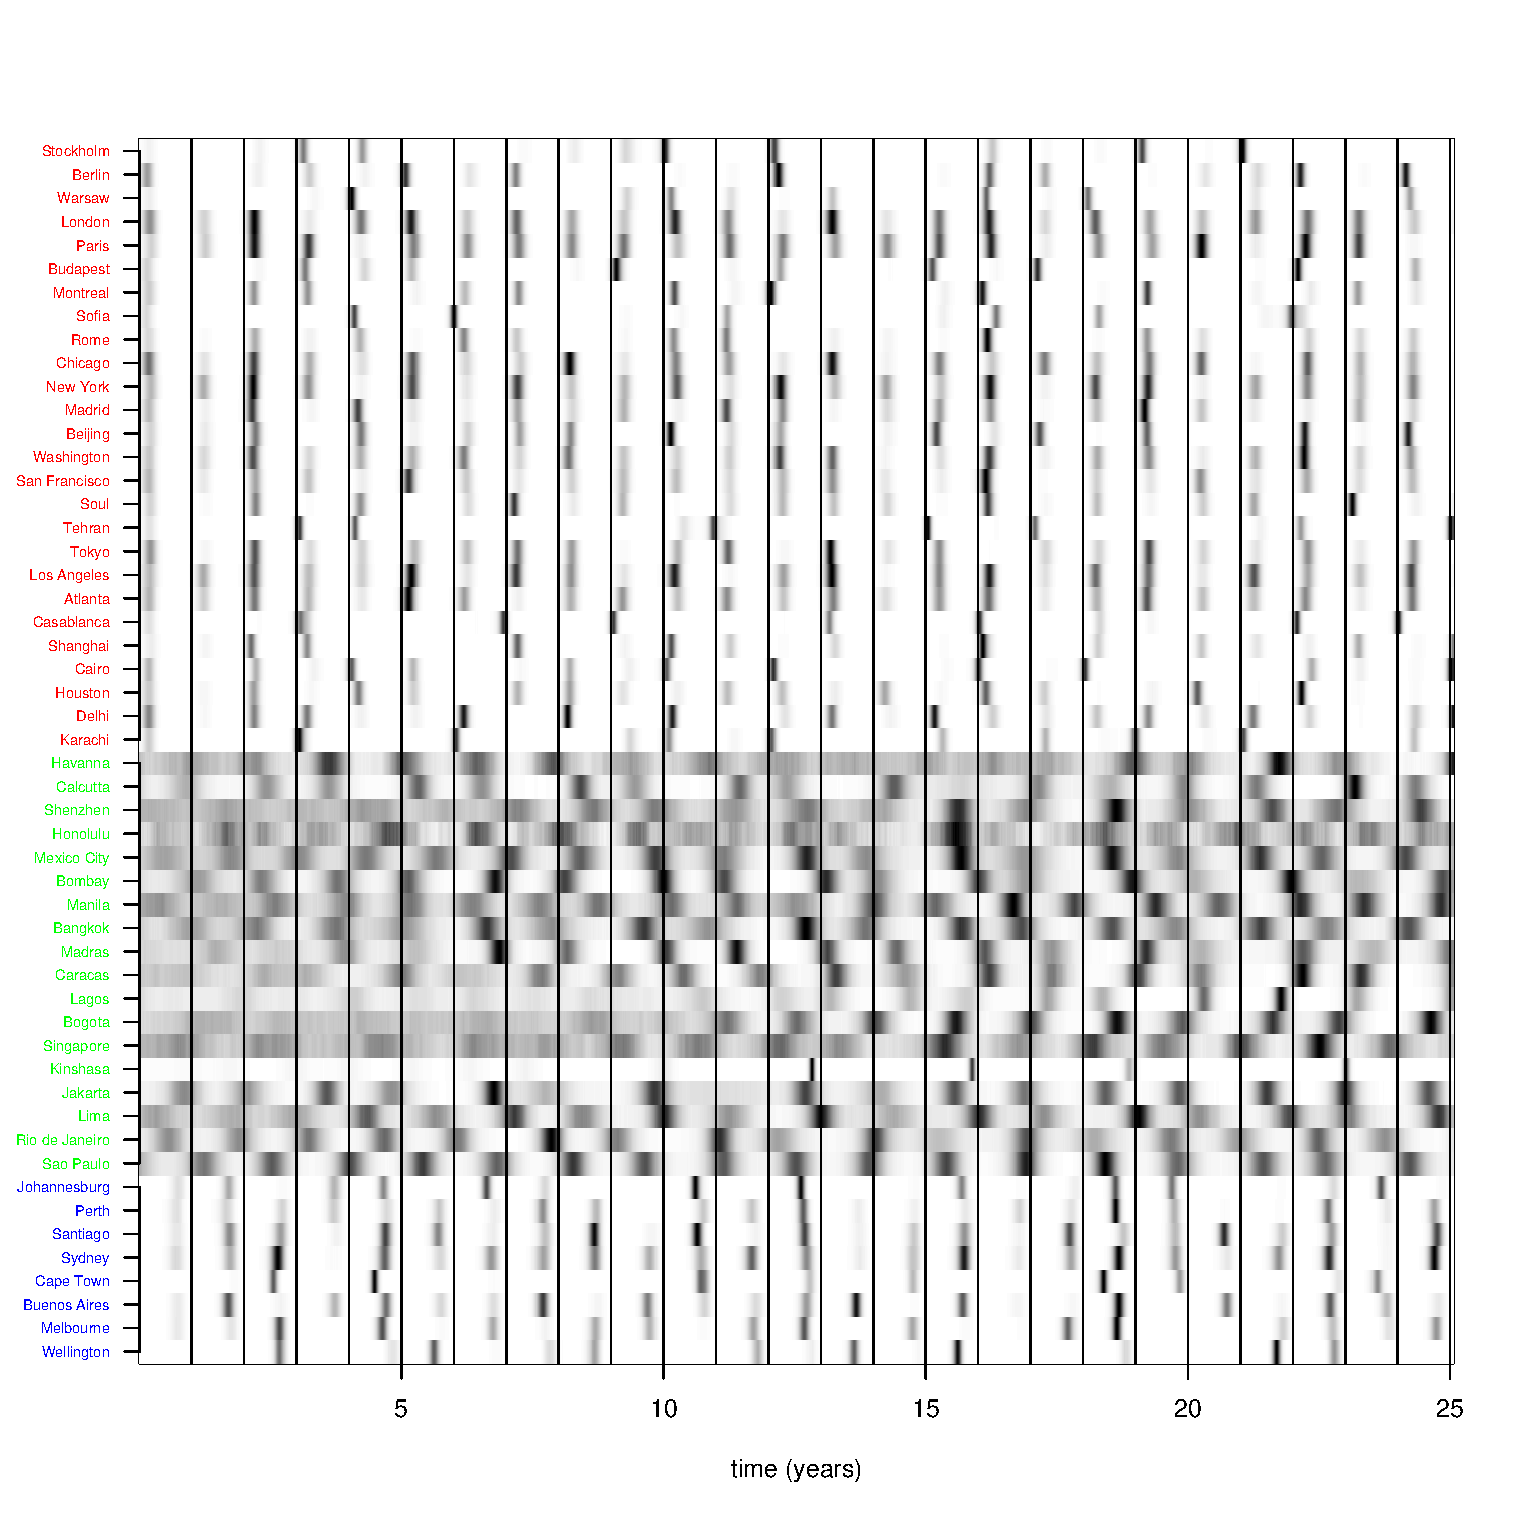
\includegraphics[width= 0.8 \linewidth]{texte/article2/graph_annexe/image_upca.eps}
  \caption{Realisations of the stochastic
    metapopulation model for each city in the metapopulation. City names are color coded by geographic area
    with red for North, green for Tropics and blue for South. Each line represents the ratio of weekly
    incidence per 100 000 inhabitant over its maximum value.
    Parameters are identical to Fig.~\ref{fig:world_aggreg}.}
  \label{fig:image_upca}
\end{figure}

\begin{figure}[htb]
  \center
  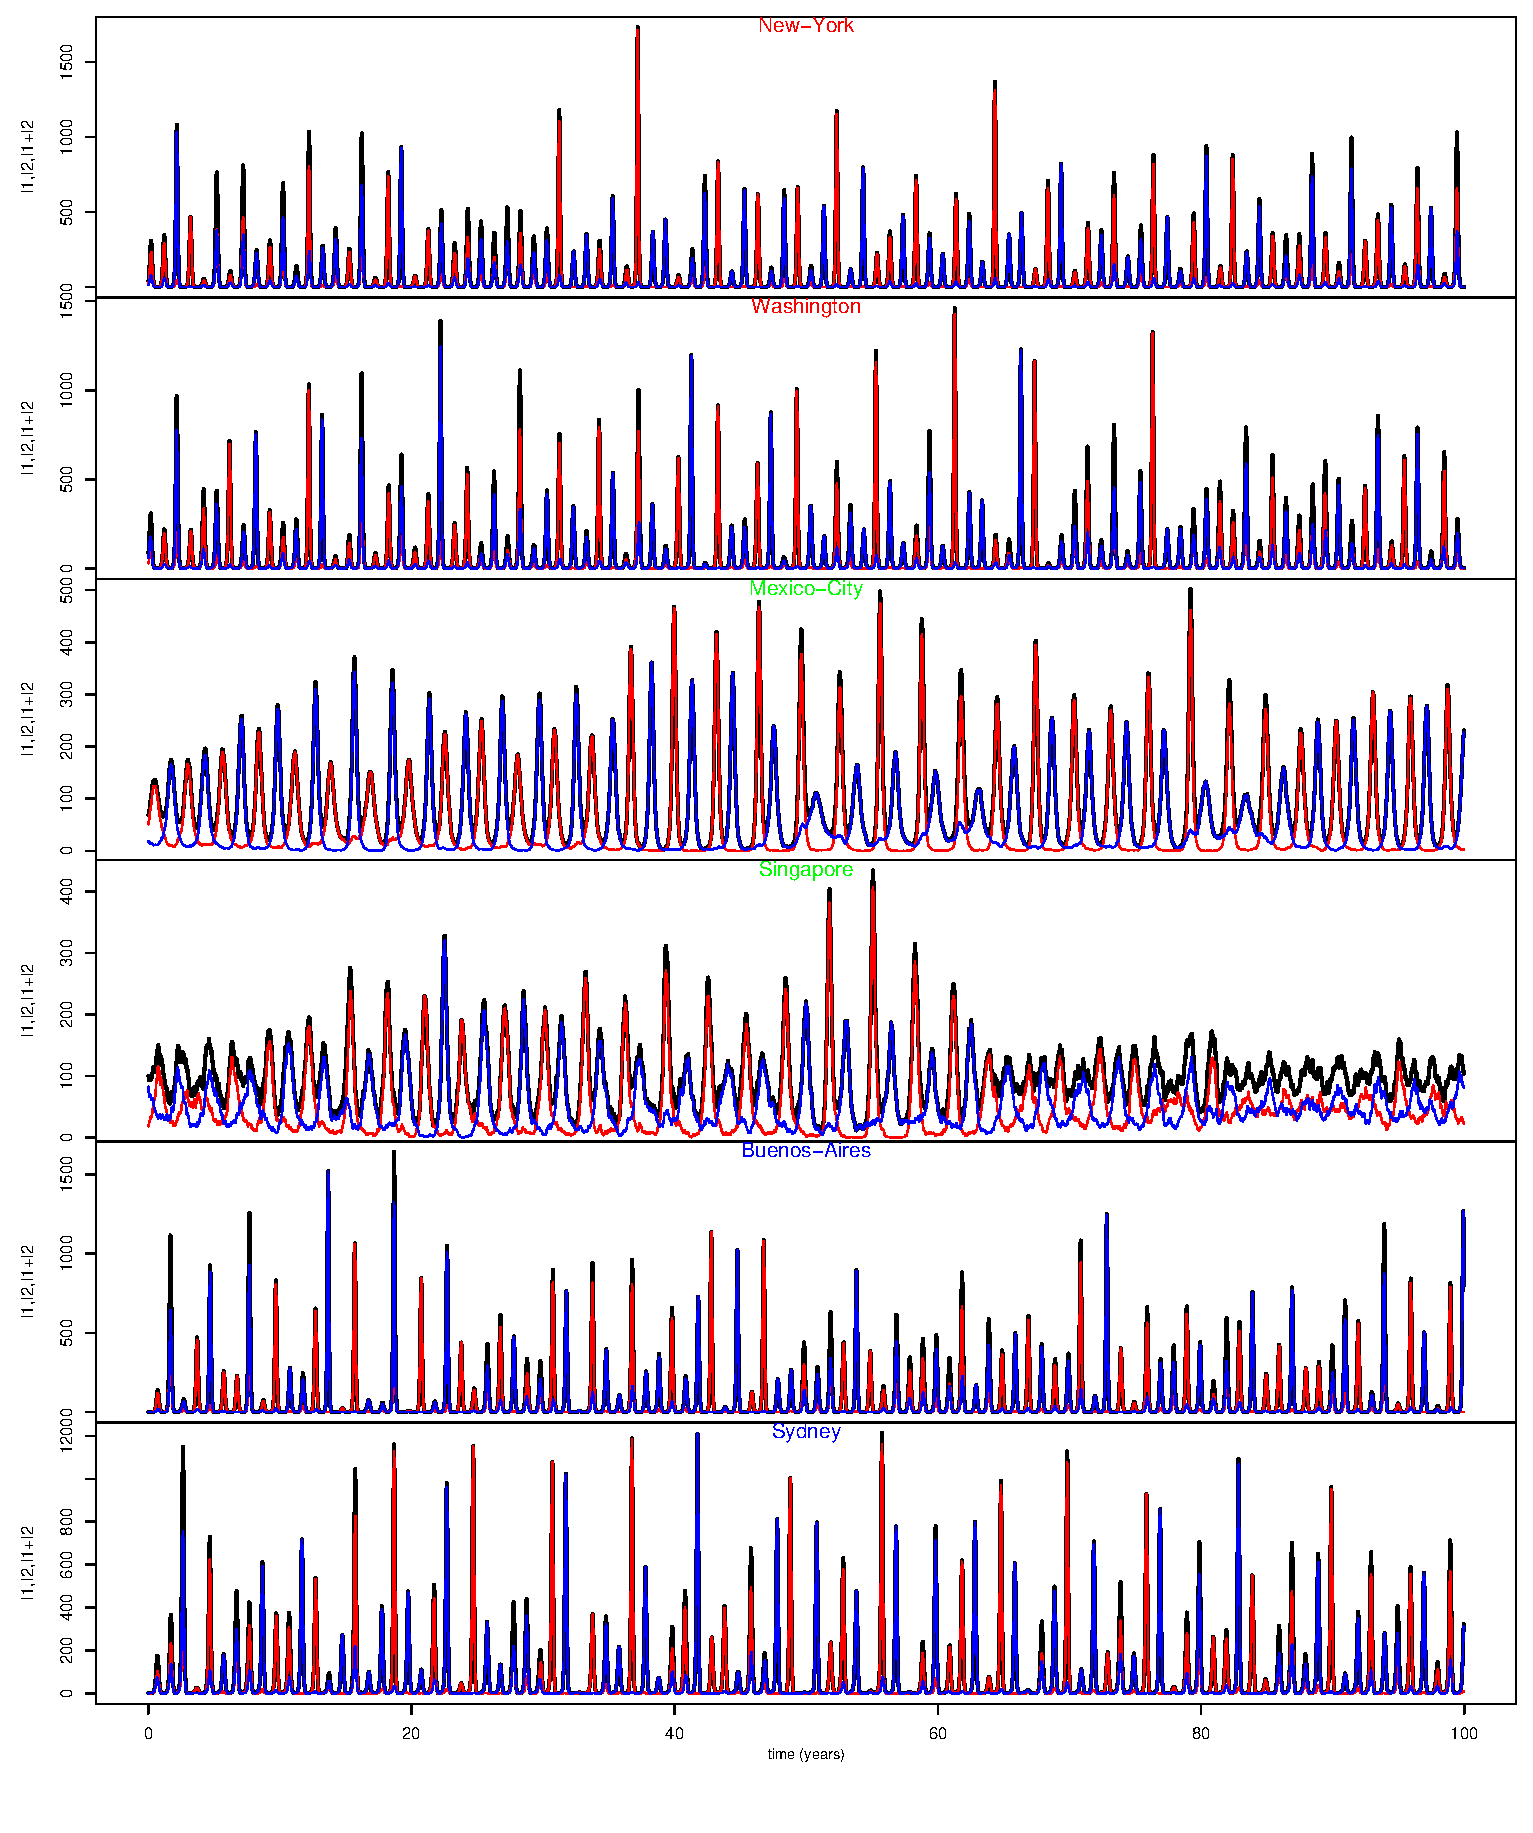
\includegraphics[width= 0.8 \linewidth]{texte/article2/graph_annexe/traj_upca_metapop.eps}
  \caption{Example of trajectories obtained in different cities from the
    three geographic areas (North, Tropics and South). Blue and red lines
    are weekly incidence per 100 000 inhabitant for subtype 1 and 2
    respectively and black lines represent the sum of both. Parameters are identical to
    figure~\ref{fig:world_aggreg}.}
  \label{fig:traj_upca_metapop}
\end{figure}


\clearpage

\section{Periods bifurcations}

\begin{figure}[htb]
  \center
    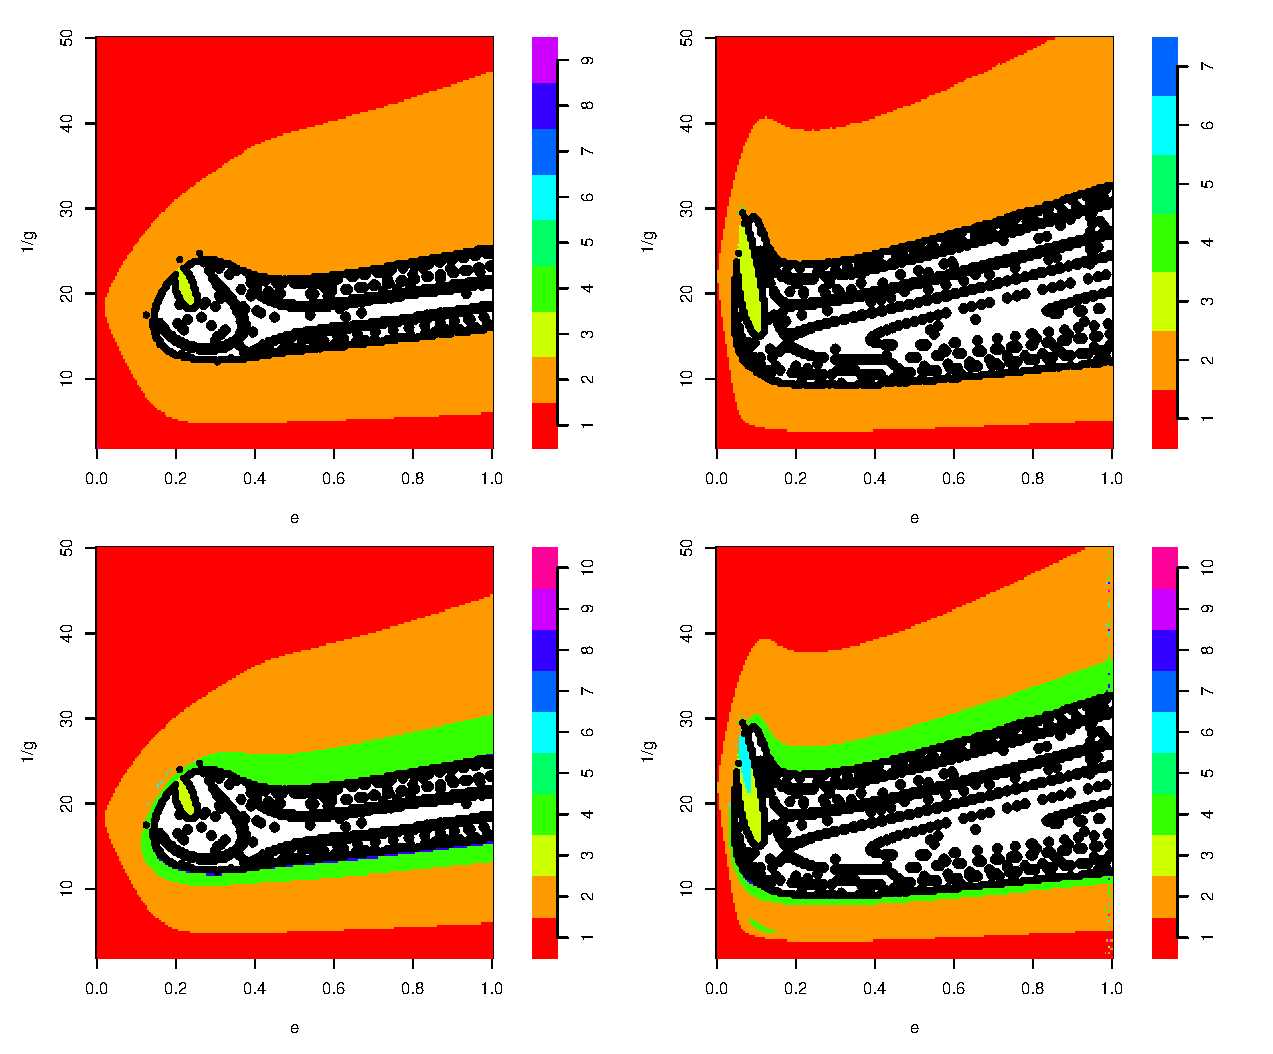
\includegraphics[width= 0.8 \linewidth]{texte/article2/graph_annexe/period1.eps}
    \caption{Bifurcation diagram for the single subtype model of
      Fig. 3 (main manuscript). Two different measures of periodicity are
      represented. Measure 1: period bifurcation is determined as the
      smallest $T$ for which $|log(I(t+T)-log(I(t))|< \epsilon$, where
      $\epsilon$ is a small numerical tolerance. Measure 2: period bifurcation is
      determined by the analysis of Fourier spectra. As the annual
      signature of seasonal forcing is always present, an arbitrary
      parameter $\epsilon'$ was used to consider that other periods are
      insignificant. Left and right graphs correspond to
      theoretical and empirical parameter sets respectively. Top and bottom graphs
       correspond to measures 2 and 1 respectively.}
  \label{fig:period1}
\end{figure}

\begin{figure}[htb]
  \center
    \includegraphics[width= 0.8 \linewidth]{texte/article2/graph_annexe/period2.eps}
    \caption{Same legend as for Fig.~\ref{fig:period1} for the two
      subtypes model of Fig.~3 (main manuscript). The periodicity of
      I1+I2 is plotted.}
  \label{fig:period2}
\end{figure}


\begin{figure}[htb]
  \center
    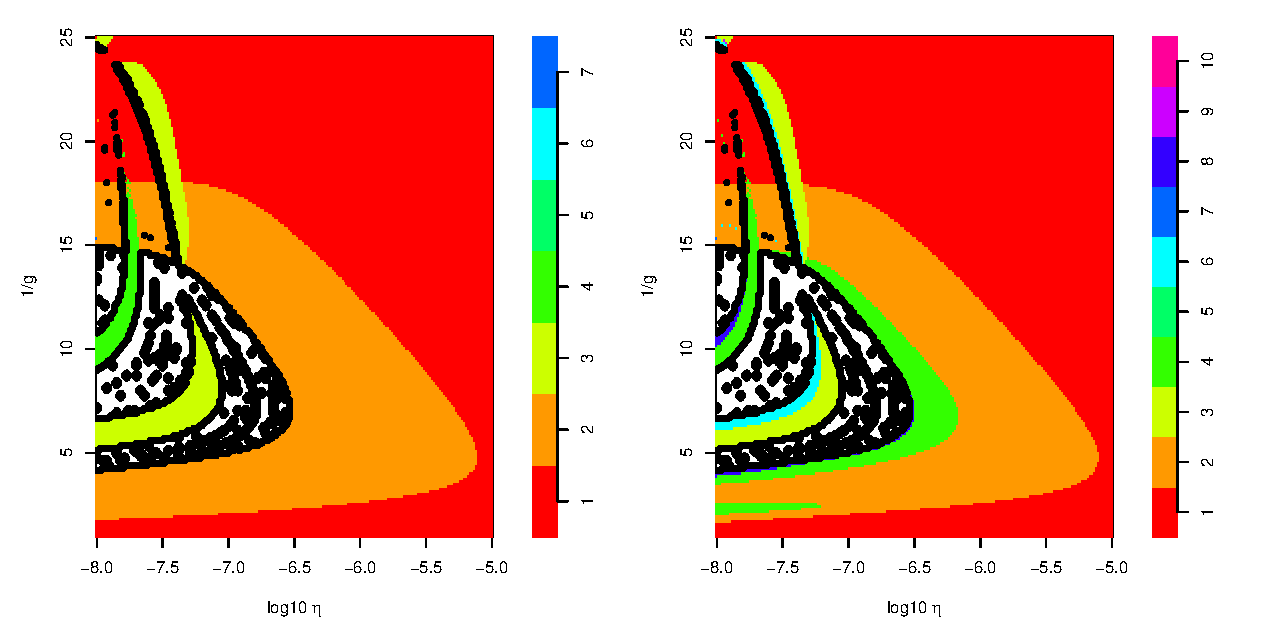
\includegraphics[width= 0.8 \linewidth]{texte/article2/graph_annexe/period_bestfit.eps}
    \caption{Same legend as for figure~\ref{fig:period1} for the
      single subtype model of Fig.~4 (main manuscript). Left and right
      graphs illustrate periods as measured by measure 2 and 1
      respectively (see caption of Fig.~\ref{fig:period1} for measures
      definition).}
  \label{fig:peiod1best}
\end{figure}

%%% Local Variables: 
%%% mode: latex
%%% TeX-master: "../../phD"
%%% End: 
